\graphicspath{{./results/}}

\chapter{Results}
% {{{
\label{cha:results}

This chapter presents the results for the quantisation experiment. Section
\ref{sec:results_methodology} details the approach taken to analysing the
various data. Section \ref{sec:results_results} presents the results from
analysing the data. The results are discussed in Section
\ref{sec:results_discussion}. Finally, Section \ref{sec:results_summary}
summarises this chapter.

Data from the different datasets in the quantisation experiment is first
presented and analysed. Finally the data from the experiment is aggregated to
provide for a more general analysis on the perception of quantisation.

\section{Methodology}
% {{{
\label{sec:results_methodology}

To analyse the responses from the experiment, a series of statistical tests are
conducted on the data to determine various statistical properties.

\paragraph{Shapiro-Wilks Test}
The first test is for normality. Further tests conducted on the data depend on
whether the data is normal or not, thus it is important to determine the
normality of the data. The hypothesis and null hypothesis of the Shapiro-Wilks
Test are: \\ \\
\textbf{Hypothesis:} The data is a normal distribution. \\
\textbf{Null hypothesis:} The data is not a normal distribution.

\paragraph{Friedman Test}
Determining if the datasets have an impact on the perceived differences for a
specific quantisation level needs to be undertaken. However, we discovered that
some the dataset specific data does not form a normal distribution. Hence,
non-parametric statistical analysis will need to be conducted.

If the data is not normal, the Friedman Test can be used to determine if the
factors have a statistically significant impact on the data. For this
experiment, the hypothesis and null hypothesis are: \\ \\
\textbf{Hypothesis:} The datasets used have an impact on the results. \\
\textbf{Null hypothesis:} The datasets do not have impact on the results.

\paragraph{ANOVA}
The aggregated data for the different quantisation levels and visualisation
techniques does form a normal distribution. Hence, parametric analysis of
the data can be used.

If the data is normal, then the Analysis of Variance (ANOVA) test can be
applied to determine if the factors have a statistically significant impact on
the data. For this experiment, the hypothesis and null hypothesis are: \\ \\
\textbf{Hypothesis:} Quantisation level has an impact on the perceived
difference between the unquantised and quantised data. \\
\textbf{Null hypothesis:} Quantisation level does not have an impact on the
perceived difference between the unquantised and quantised data.

\paragraph{Tukey's HSD}
An ANOVA analysis only indicates whether the factors have a significant impact
on the data or not. To compare the factors (the different quantisation levels),
Tukey's HSD (Honestly Significant Difference) test can be used. Tukey's HSD
does pair-wise comparisons of the resulting means for each of the factors,
indicating how similar the results are.

\paragraph{Box and whisker plot}
To graphically depict the differences between the factors, a box and whisker
plot can be used. The effect of the box and whisker plot is similar to Tukey's
HSD in that it is possible to see the individual factors and compare them to
one another.

A box and whisker plot splits the data into quartiles, and uses a box to
indicate where the first and third quartiles are. A solid line is drawn for the
second quartile, which is the median of the dataset. The whiskers of the
diagram are used to connect the smallest non-outlier to the first quartile, and
the largest non-outlier to the third quartile. Any outliers in the data are
plotted and displayed separately.

% }}}

\section{Results}
% {{{
\label{sec:results_results}

\subsection*{Dataset specific}
% {{{
\label{sub:results_results_dataset}

Four datasets were used for the experiment. As there were 30 participants, and
each participant viewed two datasets, each dataset was viewed a total of 15
times.

After performing the Shapiro-Wilks test for each of the dataset specific
results, we discovered that the null hypothesis could not be rejected for some
of the results. i.e. some of the results do not form a normal distribution.
Table \ref{tab:appendix_dataset_normality} in Appendix \ref{cha:tables} details
the test results for all the separate datasets and quantisation levels. It is
possible that the data does not form a normal distribution due to insufficient
sampling. 15 data points may not be sufficient to accurately capture the
distribution.

As not all the data follows a normal distribution, the Friedman Test was
performed. The results from the test (Table
\ref{tab:appendix_dataset_friedman}) indicate that the null hypothesis cannot
be rejected for all the data, i.e. the different datasets do not have a
significant impact on the results. The only exception to this is for the
ball-and-stick visualisation technique, using 10 bit quantisation. The reason
for this exception is unknown.

Since the datasets do not have a significant impact on the results, the results
from individual datasets can be combined. Allowing for a more general analysis
of the results.

Plotting the results on a box and whisker plot (Figures
\ref{fig:results_boxwhisker_dataset_ballstick} and
\ref{fig:results_boxwhisker_dataset_metaballs}); shows that the results are
generally quite similar. The largest variations within quantisation levels are
for the metaballs visualisation technique. However, while the results do
differ, they do not contradict each other.

\begin{figure}
  \begin{center}
    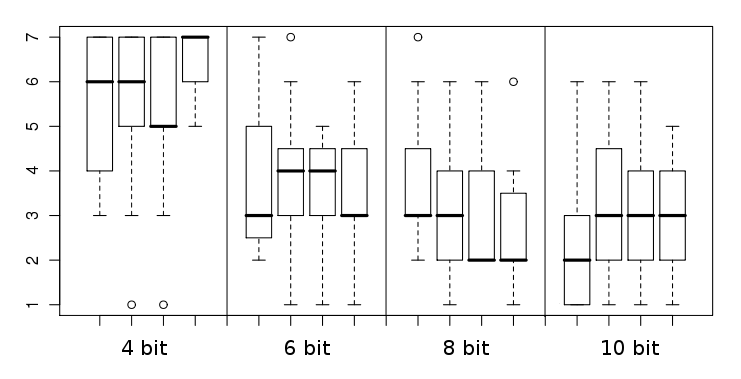
\includegraphics[width=120mm]{boxwhisker_dataset_ballstick}
  \end{center}
  \caption{Box and whisker plot of the different quantisation levels for the
  ball-and-stick visualisation. The results are very similar.}
  \label{fig:results_boxwhisker_dataset_ballstick}
\end{figure}

\begin{figure}
  \begin{center}
    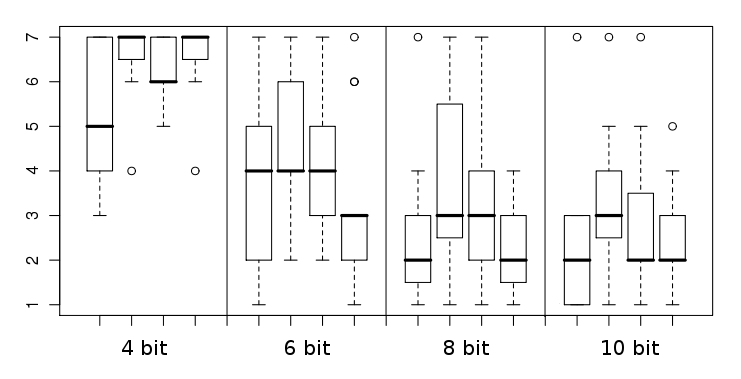
\includegraphics[width=120mm]{boxwhisker_dataset_metaballs}
  \end{center}
  \caption{Box and whisker plot of the different quantisation levels for the
  metaballs visualisation technique. The results are different, but they do
  agree with each other.}
  \label{fig:results_boxwhisker_dataset_metaballs}
\end{figure}

% }}}

\subsection*{Aggregated}
% {{{
\label{sub:results_results_aggregated}

Using the Shapiro-Wilks test for normality on the aggregated data for the ball
and stick, and metaballs visualisation techniques, the null hypothesis of the
Shapiro-Wilks test can be rejected at the 95\% significance level; i.e. the
data is a normal distribution. See Tables
\ref{tab:appendix_ballstick_normality} and
\ref{tab:appendix_metaballs_normality} in Appendix \ref{cha:tables} for the
actual test results.

With the data being verified as a normal distribution, an ANOVA analysis can be
performed. The result from ANOVA analysis indicates that the null hypothesis of
the ANOVA analysis can be rejected at the 99\% significance level, i.e.
quantisation does have a significant perceptual impact. The actual test results
is provided in Tables \ref{tab:appendix_ballstick_anova} and
\ref{tab:appendix_metaballs_anova}.

Tables \ref{tab:appendix_ballstick_tukeyhsd} and
\ref{tab:appendix_metaballs_tukeyhsd} shows the results from performing the
Tukey's HSD analysis on the results from the ball-and-stick, and metaballs
experiments, respectively. The leftmost column shows which of the quantisation
levels are being compared. For ball-and-stick, b4 means quantisation using 4
bits, b6 is 6 bit quantisation, b8 and b10 use 8 and 10 bits, respectively.
Similarly: m4, m6, m8 and m10 means quantisation levels using 4, 6, 8 and 10
bits for the metaballs visualisation technique. The difference between the
means is under the \emph{diff} column, with the lower and upper quartiles in
\emph{lwr} and \emph{upr}, respectively. \emph{p adj} indicates how similar the
factors being compared are.

Inspecting the \emph{p adj} column, 8 and 10 bit quantisation are very similar
(p-value of 0.7135299 and 0.9762546). For between 6 and 8 bit quantisation, the
ball-and-stick visualisation is similar (p-value of 0.2163136) but the values
are significantly different for the metaballs visualisation (p-value of
0.0005950). Using 4 bit quantisation, the values are significantly different
from all the other quantisation levels (p-value of 0.0000000).

Figure \ref{fig:results_boxwhisker_all} is a box and whisker plot showing the
different quantisation levels. The ball-and-stick results are on the left half
of the figure, while the right half is for the metaballs technique. The figure
reflects data from the Tukey's HSD analysis, with 8 and 10 bit quantisation
being similar, 6 and 8 bit less so, and 4 bit quantisation being different from
all the other quantisation levels.

Looking at the box and whisker plot (Figure \ref{fig:results_boxwhisker_all}),
the participants rated 4 bit quantisation as being very different from the
original (median rating of 6 and 7), 6 bit is rated different (median rating of
4), 8 and 10 bit quantisation is rated moderately different (median rating of
3).

\begin{figure}
  \begin{center}
    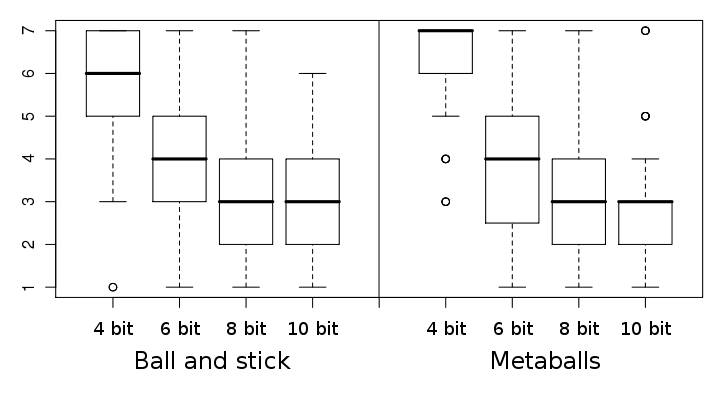
\includegraphics[width=120mm]{boxwhisker_all_both}
  \end{center}
  \caption{Box and whisker plot of the different quantisation levels.}
  \label{fig:results_boxwhisker_all}
\end{figure}

% }}}

% }}}

\section{Discussion}
% {{{
\label{sec:results_discussion}

\subsection*{Dataset specific}
% {{{
\label{sub:results_discussion_dataset}

As mentioned in Section \ref{sub:results_results_dataset}, the Friedman
Test indicates that the different datasets do not have a significant impact on
the results. This means that the perceptually visible effects of quantisation
are similar between datasets.

The effects are not exactly equal due to the size differences in the datasets.
As quantisation produces a limited number of possible values which can be used,
a dataset with larger dimensions will have larger quantisation errors, and thus
more noticeable differences.

However, for datasets with fewer molecules, the bounding box of the data can
shift around as the molecules move. With more molecules, the bounding box is
more likely to remain still as more molecules will need to move in a certain
direction to shift the bounding box. As quantisation allocates values equally
across the bounding box, a shift in the bounding box would cause a
corresponding shift of all the values. In the visualisation, this would be
characterised as the entire volume of data moving around. The simulation would
appear ``wobbly''. The wobbling is more noticeable with quantisation using
fewer bits.

In further analysing the data, there is no consistent increase or decrease in
the noticeable difference with regards to datasets. This may have been as a
result of a number of factors:
\begin{itemize}

  \item participant uncertainty: different participants have their own
  different definitions of ``similar'' and ``different''.

  \item participant bias: participants can be naturally inclined towards
  perceiving similarities, or differences, hence biasing their results.

  \item the quantisation levels were shown in a random order; this may
  influence the participants' short-term memory, and thus impact on the
  perceived differences.

  \item large datasets have greater quantisation errors, but the smaller
  datasets ``wobble'', there is thus a visual difference either way.

\end{itemize}

While there are differences as a result of the datasets, the differences are
small and the responses are consistent across datasets.

% }}}

\subsection*{Aggregated}
% {{{
\label{sub:results_discussion_aggregated}

As the dataset does not have a significant impact on the results, all the
results for a specific quantisation level and visualisation technique can be
combined and aggregated together. This allows for a more general analysis of
the effects of quantisation.

The responses from the experiment indicate that 8 and 10 bit quantisation yield
similar results, 6 bit is still similar (but less so), with 4 bit being very
different from the original data. This does reflect the effects of
quantisation. As fewer bits are used, exponentially fewer values are available.
10 bits allows for 1024 possible values, but 4 bits only allows for 16 possible
values. This applies separately to each coordinate. See Table
\ref{tab:results_bitvalues} for an indication of the number of possible values
for each of the quantisation levels.

\begin{table}
  \begin{tabular}{ | l | r | }
  \hline
  Quantisation level & Number of values  \\ \hline
  4 bit              &               16  \\ \hline
  6 bit              &               64  \\ \hline
  8 bit              &              256  \\ \hline
  10 bit             &             1024  \\ \hline
  \end{tabular}
  \caption{Table showing number of values per quantisation level}
  \label{tab:results_bitvalues}
\end{table}

Plotting the means of the quantisation levels (Figure
\ref{fig:results_bm_means}) shows that the metaballs visualisation technique
yields more noticeable differences when using fewer bits, than that of
ball-and-stick.

\begin{figure}
  \begin{center}
    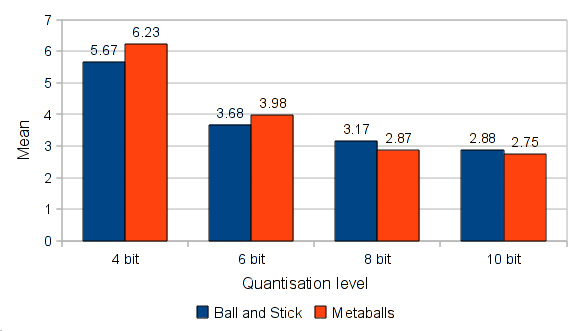
\includegraphics[width=100mm]{bm_means}
  \end{center}
  \caption{Graph showing the mean values of the different quantisation levels}
  \label{fig:results_bm_means}
\end{figure}

As the ball-and-stick visualisation technique shows the individual atoms, it is
easier to see the differences between the original and quantised data. The
spheres are at the actual quantised positions, and quantisation will result in
the spheres being placed in a different position, which is easily noticed.

Due to how the metaballs surface is extracted, the quantisation effects are
very noticeable when using fewer bits. As fewer bits are used, there will be
fewer positions for the water molecules. This distorts the areas of water and
non-water. The resulting extracted surfaces highlight the quantised positions.
See Figure \ref{fig:experiment_metaballs4680}, the quantised water positions
are clearly visible when using 4 bit quantisation.

The quantised water positions are not as clearly visible when using more bits
as the water molecules are placed more accurately, and the water molecules do
not overlap as much.

The metaballs surface is determined by the nearby water molecules, which means
that slight variations in the water molecule positions will not be clearly
reflected in the surface. This explains why the 8 and 10 quantisation levels
are so similar.

% }}}

% }}}

\section{Summary}
% {{{
\label{sec:results_summary}

The statistical analysis shows that the datasets do not have a significant
impact on the results, meaning that the results between datasets are comparably
similar.

Aggregating data from the different datasets together, and analysing this shows
that quantisation levels do have a statistically significant impact on the
perceived difference.

At quantisation levels using fewer bits, the metaballs visualisation technique
is more visually different than that of the ball-and-stick visualisation
technique. Conversely, the ball-and-stick ratings for quantisation levels using
more bits are higher; i.e. the difference from the original data is greater.

Since the perceived difference between 8 and 10 bit quantisation levels is not
statistically significant, 8 bit quantisation is the recommended quantisation
setting. If the data to be compressed is very large, more bits per quantisation
may be needed. However, for data used purely for viewing, 8 bit quantisation is
sufficient.

% }}}

% }}}

